\section{Android}

Perusjutut androidista.

\subsection{Historia}

Androidin kehityksen aloitti Android Inc. -niminen yritys vuonna 2003. Google osti sen vuonna 2005. Kaksi vuotta myöhemmin, marraskuussa 2007 Androidin ensimmäinen versio julkaistiin ja samalla kerrottiin, että sen kehityksestä vastaa Open Handset Alliance, johon kuului Googlen lisäksi puhelinvalmistajia, kuten HTC ja Samsung, operaattoreita, kuten Sprint Nextel ja T-Mobile sekä komponenttivalmistajia, kuten Qualcomm ja Texas Instruments.

Ensimmäinen Androidille julkaistu kaupallinen laite oli HTC Dream -älypuhelin, joka julkaistiin lokakuussa 2008.
Loppuvuodesta 2010 Android nousi älypuhelinten markkinajohtajaksi. Syksyllä 2012 Androidilla oli jo tutkimuksesta riippuen 50-70 prosentin markkinaosuus ja laitevalikoima on kasvanut älypuhelimista muunmuassa tablet-tietokoneisiin, digibokseihin ja kameroihin.\cite{wikiandroid}

Tähän vähän kattavammin jotain..

\subsection{Ihan perusteet}

Android-sovelluksia tehdään Java-ohjelmointikielellä. Google julkaisee ilmaista SDK:ta (suomennos!), joka kääntää sovelluksen ja pakkaa sen kuvien ja muiden resurssien kanssa apk-tiedostoksi, joka sisältää yhden sovelluksen kaiken tiedon. Sitä käytetään myös sovelluksen asentamiseen Android-puhelimeen.

Android on rakennettu Linuxin ytimen version 2.6 päälle. Jokainen sovellus on oma käyttäjänsä järjestelmässä ja sovellusten oikeudet on rajattu siten että ne pääsevät käsiksi vain kyseiseen sovellukseen liittyviin resursseihin. Lisäksi jokainen sovellus pyörii omassa virtuaalikoneessaan eristettynä muista sovelluksista. Jokaisella sovelluksella on oma prosessinsa, jota Android hallitsee sovelluksen elinkaaren ajan. Androidin perusturvallisuusratkaisu noudattaa principle of least privilegeä (suomennos). Sovelluksella on vain ne oikeudet, joita se vähintään tarvitsee toimintaansa. Kaikkia ylimääräisiä oikeuksia varten täytyy erikseen pyytää lupa.

Android-sovellukset koostuvat neljän tyyppisistä komponenteista: aktiviteeteista (activities), palveluista (services), sisällöntarjoajista (content providers) sekä lähetysten vastaanottajista (broadcast receivers).

Aktiviteetti kuvaa yhtä sovelluksen näkymää. Sovelluksen käyttöliittymä koostuu useista aktiviteeteista, jotka muodostavat yhdessä koherentin sovelluksen, mutta jokainen aktiviteetti on toisistaan riippumaton. Eri sovellukset voivat myös käynnistää toistensa aktiviteetteja, mikäli vastaanottava sovellus sen sallii. Esimerkiksi kamera-sovellus voi käynnistää sähköposti-sovelluksen sähköpostinkirjoitus-aktiviteetin, jos ottamansa kuvan haluaa jakaa sähköpostilla. Aktiviteetit ovat Androidissa Activity-luokan aliluokkia.

Palvelut ovat taustaprosesseja, jotka suorittavat pitkäkestoisia operaatioita, kuten tiedon lataamista verkosta tai musiikin soittamista taustalla samalla kun käyttäjä käyttää toista sovellusta. Palvelut eivät tarjoa käyttöliittymää ja toiset komponentit, kuten aktiviteetit, voivat käynnistää niitä. Palvelut ovat Service-luokan aliluokkia.

Sisällöntarjoajat vastaavat sovelluksen tarvitseman tiedon lukemisesta ja kirjoittamisesta pitkäkestoiseen muistiin. Tallennuspaikkana voi olla laitteen tiedostojärjestelmä, SQLite-tietokanta, verkko tai ylipäänsä mikä tahansa kohde, johon sovelluksella on luku tai kirjoitusoikeudet. Sovellukset voivat käyttää toistensa sisällöntarjoajia mikäli sovellus julkaisee ne muiden sovellusten käyttöön. Sisällöntarjoajat toteuttavat ContentProvider-rajapinnan, joka mahdollistaa transaktiot datan kirjoittamiseen ja lukemiseen.

Lähetysten vastaanottajat reagoivat järjestelmänlaajuisiin viesteihin ja tapahtumiin. Tällaisia ovat esimerkiksi ilmoitus, että patteri on lopussa, tai että käyttäjä on sulkenut tai avannut näytön. Ne voivat myös lähettää järjestelmänlaajuisia tapahtumaviestejä muille sovelluksille. Lähetysten vastaanottajat ovat BroadcastReceiver-luokan aliluokkia, ja tapahtumat ovat Intent-luokan aliluokkia.

Android-sovellukset käyttävät usein hyväkseen toisten sovellusten komponentteja. Sovellukset eivät pysty suoraan kutsumaan toisiaan, vaan halutessaan hyödyntää toisten sovellusten ominaisuuksia sovellus luo uuden aikeen, jonka järjestelmä välittää tiettyjen sääntöjen perusteella sopivalle vastaanottajalle (katso luku \ref{intents}). Koska aikeet voivat käynnistää sovelluksesta monia eri komponentteja, Android-sovelluksilla ei ole yksittäistä main-metodia, joka käynnistäisi ohjelman, kuten usein muissa sovelluksissa on tapana. \cite{android}

\subsection{Aktiviteetit}

\begin{figure}[htb]
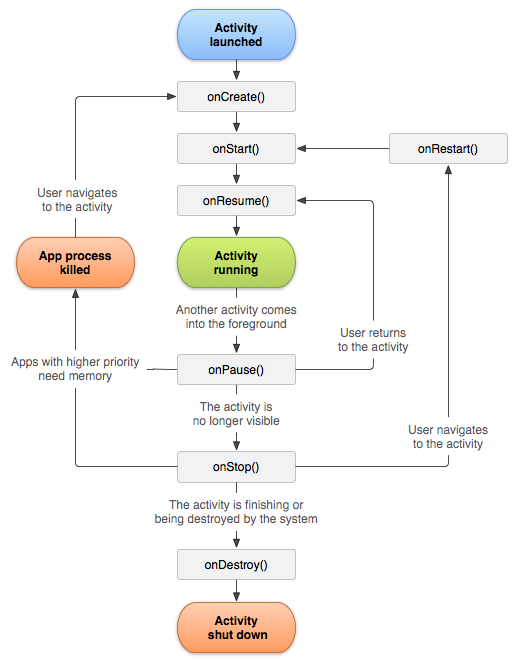
\includegraphics[width=100mm]{activity_lifecycle.png}
\caption{placeholder omalle kuvalle} \label{activity_lifecycle}
\end{figure}

Aktiviteetit kuvaavat yhtä sovelluksen näkymää. Tyypillisesti aktiviteetti on koko näytön kokoinen, mutta ne voivat olla myös pienempiä tai leijua osittain toisen aktiviteetin päällä. Yksi sovelluksen aktiviteeteistä on yleensä pääaktiviteetti, joka käynnistyy silloin, kun käyttäjä avaa sovelluksen. 

Aktiviteettien elinkaaren hallinta on Android-sovelluksen kriittisimpiä osia, koska järjestelmän resurssit ovat yleensä hyvin rajalliset ja Android-laitteiden käyttöön liittyy usein tiheä vaihtelu eri sovellusten välillä. Tällöin on tärkeää, että sovellus luovuttaa varaamansa resurssit muiden sovellusten käyttöön kun sovellus vaihtuu ja vastaavasti osaa palautua takaisin pysäytettäessä olleeseen tilaan käyttäjän palatessa sovellukseen. Nämä vaihdokset pitäisi lisäksi tapahtua mahdollisimman tehokkaasti, että järjestelmän toiminta olisi käyttäjän näkökulmasta mahdollisimman sulavaa sovellusten tilojen vaihtamisen yhteydessä.

Aktiviteetilla voi olla pitkäkestoisemmin kolme eri tilaa. Aktiviteetti on aktiivisessa tilassa (resumed) silloin kun se on näytön etualalla ja käyttäjä käyttää juuri sitä aktiviteettia. Keskeytetyssä (paused) tilassa aktiviteetti on, kun se on osittain näkyvissä, mutta jokin toinen aktiviteetti on aktiivisena sen päällä. Keskeytetyt aktiviteetit ja niiden tilat pysyvät muistissa, joskin jos laitteen muisti on äärimmäisen lopussa, järjestelmä saattaa tuhota sen. Aktiviteetti on pysäytetty (stopped) silloin, kun jokin toinen aktiviteetti peittää sen kokonaan näkyvistä. Tällainenkin aktiviteetti säilyy muistissa, jos laitteen resurssit ovat riittävät, mutta järjestelmä voi tuhota sen koska vain, jos resursseja tarvitaan muiden aktiviteettien käyttöön.

Aktiviteetin siirtyminen eri tilojen välillä tapahtuu järjestelmän kutsuessa aktiviteetin callback-metodeita (suomennos?). Mahdolliset tilasiirtymäpolut näkyvät kuvassa \ref{activity_lifecycle}. 

Aktiviteetin koko elinkaari tapahtuu onCreate()- ja onDestroy()-kutsujen välillä. Aktiviteetin tulisi tehdä kaikki kerran suoritettavat globaalit tilanalustustehtävät kutsuttaessa onCreate()-metodia, kuten ulkoasun määrittely tai koko aktiviteetin elinkaaren ajan tarvittavan tiedonsiirtosäikeen avaus. Vastaavasti onDestroy()-kutsussa aktiviteetin tulisi vapauttaa kaikki loputkin aktiviteetin varaamat resurssit.

Aktiviteetin käyttäjälle näkyvä elinkaari on onStart()- ja onStop()-kutsujen välillä. onStart()-metodia kutsutaan kun aktiviteetti tulee näkyväksi käyttäjälle ja onStop()-metodia kutsutaan kun jokin toinen aktiviteetti on peittänyt kyseisen aktiviteetin kokonaan. Näkyvän elinkaaren aikana tulisi ylläpitää niitä resursseja, joita tarvitaan käyttäjän kanssa kommunikointiin sekä sellaisia, jotka saattavat muuten vaikuttaa käyttäjälle näkyvään käytöliittymään. Esimerksiki lähetystenvastaanottajaa on hyvä kuunnella tällä välillä mahdollisten järjestelmänlaajuisten käyttöliittymään vaikuttavien tapahtumien varalta. onStart() ja onStop() -kutsuja voi tulla lukuisia aktiviteetin koko elinkaaren aikana. onRestart()-metodia kutsutaan, jos aktiviteetti on jo luotu aiemmin ja pysäytetty sitten onStop()-kutsulla. onRestart()-kutsua seuraa aina onStart()-kutsu.

Aktiviteetti on aktiivisena näytön etualalla onResume() ja onPause() -kutsujen välillä. Kun aktiviteetti on etualalla, käyttäjä käyttääj uuri sitä ja se on kaikkien muiden aktiviteettien päällä. onResume() ja onPause() -kutsuja voi tulla tiheästi, esimerkiksi aina kun laitteen näyttö menee lepotilaan tai tulee jokin ilmoitus aktiviteetin päälle, joten onResume() ja onPause() -metodien tulisi olla kevyitä.

Androidin järjestelmä voi tuhota sovelluksen prosessin onPausen(), onStopin() tai onDestroyn() jälkeen. Tämän takia tärkeä pysyvä tieto on syytä tallentaa onPause()-kutsun jälkeen. Tallennus voidaan tehdä esimerkiksi toteuttamalla vapaaehtoinen callback-metodi onSaveInstanceDate(), jota kutsutaan aina ennen kuin järjestelmä mahdollistaa aktiviteetin tuhoamisen. onSaveInstanceData() saa parametrinaan Bundle-olion, johon voi tallentaa tietoja nimi-arvo-pareina. Sama Bundle-olio tulee aktiviteetille onCreate() ja onRestoreInstanceState() -metodeille. Tiedon palautuksen voi tehdä kummassa tahansa näistä metodeista. Activity-luokka tarjoaa myös oletustoteutuksen onSaveInstanceData()- onRestoreInstanceState()-metodeista, jotka osaavat monissa tapauksissa suorittaa tiedon tallennuksen (ja kyseisten metodien yliluokkatoteutusta onkin syytä kutsua omasta toteutuksesta). Aktiviteetin tilanpalautusta tarvitaan usein, esimerkiksi aina kun käyttäjä vaihtaa sovelluksen suuntaa pysty- ja vaakasuuntien välillä.

Aktiviteettien vaihtumisen yhteydessä takaisinkutsujen järjestys on aina sama. Kun aktiviteetti A käynnistää aktiviteetti B:n, ensin kutsutaan aktiviteetti A:n onPause()-metodia, sitten aktiviteetti B:n onCreate(), onStart() ja onResume()-metodeita peräkkäin. Viimeiseksi kutsutaan aktiviteetti A:n onStop()-metodia, mikäli aktiviteetti B peittää sen kokonaan. Näin esimerkiksi aktiviteetti A:n onPause()-metodissa tietokantaan tallennetut tiedot ovat käytössä aktiviteetti B:tä käynnistettäessä. Jos muutoksia taas tekee onStop()-metodissa, ne tapahtuvat vasta aktiviteetti B:n käynnistyttyä.

Androidin versiosta 3 (API-versio 11) asti on ollut mahdollista määritellä aktiviteetteihin fragmentteja (Fragment). Fragmentit ovat uudelleenkäytettäviä komponentteja, joita voi käyttää osana aktiviteetteja. Niiden avulla on helpompi luoda käyttöliittymiä, jotka skaalautuvat eri kokoisille näytöille. Isommalla näytöllä aktiviteetti voi pitää sisällään useita fragmentteja, jotka pienemmällä näytöllä ovatkin omissa aktiviteeteissaan. Fragmenttien elinkaari on riippuvainen siitä aktiviteetista, johon ne on sisällytetty. Kun aktiviteetti pysähtyy, niin pysähtyy myös aktiviteetin sisältämät fragmentit. Samoin aktiviteetin tuhoutuessa tuhoutuu myös fragmentit. Aktiviteettien sisällä fragmenteilla voi kuitenkin olla oma elinkaarensa, niitä voi käynnistää ja tuhota vapaasti aktiviteetin ollessa käynnissä.

Fragmenttien elinkaarta hallitaan callback-metodeilla, kuten aktiviteettejakin. Monet metoditkin ovat samoja, kuten onCreate(), onStart(), onPause() ja onStop(). Lisäksi fragmenteilla on omia callback-metodeita. onCreateView()-metodia kutsutaan, kun fragmentin käyttöliittymä tulee ensimmäistä kertaa näkyviin käyttäjälle. onAttach()-metodia kutsutaan kun fragmentti on liitetty johonkin aktiviteettiin. Tällöin fragmentti saa itselleen viitteen aktiviteettiin kommunikointia varten. onActivityCreated()-metodia kutsutaan, kun fragmentin liittäneen aktiviteetin onCreated()-metodi on ajettu. onDestroyView()-metodia kutsutaan kun fragmentin käyttöliittymä tuhotaan ja onDetach()-metodia kutsutaan kun fragmenttiin liitetty aktiviteetti irroitetaan fragmentista.

Layout-tiedostoista jotain.. Ei ehkä niin olennaista, että tarvitsisi tehdä oma aliluku.  \cite{android}

\subsection{Palvelut}

\begin{figure}[htb]
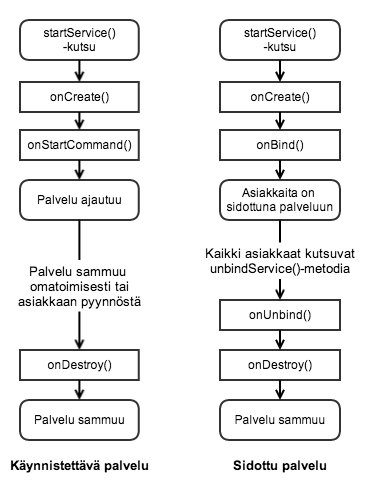
\includegraphics[width=100mm]{service_lifecycle.png}
\caption{placeholder omalle kuvalle} \label{service_lifecycle}
\end{figure}

Palvelut ovat pitkäkestoisia taustaoperaatiota. Muut sovelluskomponentit voivat käynnistää niitä ja ne jatkuvat vaikka käyttäjä lopettaisi kyseisen sovelluksen käyttämisen. Palvelu voi esimerkiksi soittaa musiikkia, suorittaa verkkotransaktioita, kommunikoida sisällöntarjoajien kanssa tai tehdä levykirjoitusta.

Palvelut voivat olla kahdenlaisia. Käynnistettävät (started) palvelut suorittavat tehtävänsä kun niiden startService()-metodia kutsutaan. Tällainen palvelu voi jatkaa pyörimistä taustalla, vaikka sovellus suljettaisiin. Tyypillisesti käynnistettävä palvelu tekee jonkin yhden operaation, kuten tiedoston latauksen tai lähettämisen, ja lopettaa sitten itsensä. Käynnistettävät palvelut eivät yleensä palauta palautusarvona kutsujalle mitään. Käynnistettävien palveluiden tulee sulkea itsensä operaation valmistuttua kutsumalla stopSelf()-metodia. Myös muut komponentit voivat sulkea palvelun kutsumalla stopService()-metodia.

Sidotut (bound) palvelut ovat sellaisia, että sovelluskomponentit sitovat palvelun niihin kutsumalla bindService()-metoida. Sidotut palvelut tarjoavat asiakas-palvelin (client service..) rajapinnan sitovalle komponentille. Palvelu voi vastaanottaa pyyntöjä ja palauttaa vastauksia niihin. Palvelun elinkaari on sama kuin sen sitoneen komponentin. Useampi komponentti voi sitoa saman palvelun yhtä aikaa. Tällöin palvelu sulkeutuu kun viimeinenkin niistä lopettaa toimintansa. Sitominen vapautetaan kutsumalla unbindService()-metodia.

Useimmiten käynnistettävät ja sidotut palvelut ovat erillisiä, mutta joissain tilanteissa sama palvelu voi toimia sekä käynnistettävänä että sidottuna palveluna. 

Palveluiden elinkaari kuvassa \ref{service_lifecycle}. Aktiviteettien tavoin koko palvelun elinkaari tapahtuu onCreate() ja onDestroy()-kutsujen välissä ja palvelun alustus tapahtuu onCreate()-metodissa. Palvelun aktiivinen elinkaari on onBind() ja onUnbind()-kutsujen välillä, tai käynnistettävän palvelun tapauksessa onStartCommand()-kutsusta kunnes se sulkee itsensä stopSelf()-kutsulla. onBind() ja onStartCommand() -metodit saavat parametrinaan aikeen, jonka niitä kutsunut komponentti antoi bindService() tai startService() -metodille. \cite{android}

\subsection{Sisällöntarjoajat}

Sisällöntarjoajat tarjoavat pääsyn pysyvästi tallennettuun tietoon. Ne kapsuloivat tiedon ja tarjoavat mekanismit tiedon yksityisyyden hallintaan. Sisällöntarjoajat toimivat rajapintana tiedon ja sovelluskoodin välillä. Kun sisällöntarjoajan tietoon halutaan päästä käsiksi, käytetään ContentResolver-oliota sovelluksen kontekstissa (Context), joka sitten kommunikoi itse sisällöntarjoajan kanssa.

Sisällöntarjoajat eivät ole välttämättä olennaisia, jos tietoon ei haluta päästä käsiksi muista kuin samasta sovelluksesta. Sovellustenväliseen kommunikointiin sisällöntarjoajat tarjoavat vakiorajapinnan, joka pitää huolen prosessienvälisestä kommunikoinnista ja tietoturvallisuudesta.

Androidin mukana tulee valmiiksi toteutetut sisällöntarjoajat esimerkiksi musiikille, videotiedostoille ja käyttäjän yhteystiedoille. Joitain rajoitteita lukuunottamatta nämä sisällöntarjoajat ovat kaikkien sovellusten käytettävissä. \cite{android}

\subsection{Aikeet}
\label{intents}

Suurin osa Android-sovellusten kommunikaatiosta on tapahtumapohjaista. Niin aktiviteetit, palvelut kuin sisällöntarjoajatkin käynnistetään lähettämällä niille aie (intent). Tapahtumia käytetään Androidissa, koska niiden avulla komponentit voidaan sitoa toisiinsa ajonaikaisesti ja vasta silloin kun niitä varsinaisesti tarvitaan. Itse aie-oliot ovat passiivisia tietorakenteita, joissa on abstrakti kuvaus operaatiosta, joka halutaan suoritettavan tai lähetysten (broadcast) tapauksessa kuvaus siitä, mitä on tapahtunut. 

Aikeiden kohde voidaan nimetä ekspliittisesti ComponentName-kentässä. Tällöin annetaan kohdekomponentin täydellinen nimi paketteineen, jolloin kohde voidaan tunnistaa yksikäsitteisesti. Tämän muodon käyttäminen vaatii, että kutsuva komponentti tietää kohdekomponentin nimen. Sovelluksensisäisessä kommunikoinnissa tämä onnistuu, mutta sovellustenvälisessä kommunikoinnissa useinkaan ei. Tällöin kohde päätellään implisiittisesti muista aikeelle annetuista kentistä.

Action-kentässä annetaan tapahtuma, joka aikeella halutaan käynnistää, esimerkiksi puhelun aloitus, tai lähetysten vastaanottajien tapauksessa järjestelmässä tapahtunut tapahtuma, kuten varoitus patterin loppumisesta. Intent-luokassa määritellään lukuisia vakioita erilaisia tapahtumia varten, mutta niiden lisäksi sovellukset voivat määritellä myös omia tapahtumia.

Data-kentässä annetaan tapahtumaan liittyvän tiedon osoite (URI) ja tyyppi (MIME). Näin vastaanottava komponentti tietää minkätyyppistä tietoa aikeeseen liittyy, ja mistä se löytyy. Category-kentässä kerrotaan, minkä tyyppisen komponentin odotetaan käsittelevän aikeen. (tähän esimerkkejä). Näitäkin Intent-luokka tarjoaa valmiita, mutta omien käyttö on mahdollista.

Aikeen vastaanottava komponentti voidaan päätellä kahdella tavalla. Jos ComponentName-kentässä on arvo, käytetään siinä määriteltyä komponenttia eikä muiden kenttien arvoista välitetä. Muussa tapauksessa Action-, Data- ja Category-kenttien arvojen perusteella selvitetään, mitä soveltuvia vastaanottavia komponentteja järjestelmään on asennettuna. Tässä käytetään apuna aiesuotimia (Intent filter).

Sovellukset voivat määritellä aiesuotimia, jotta järjestelmä tietää, mitkä sovellukset voivat ottaa vastaan aikeita. Aiesuotimet ovat komponenttikohtaisia, ja ne määrittelevät, mitä tapahtumia, tietotyyppejä ja kategorioita ne tukevat. Aiesuotimia käytetään hyväksi implisiittisessä kohteen määrittelyssä. Jos kohde on määritelty eksplisiittisesti komponentin nimellä, aiesuotimilla ei ole vaikutusta. \cite{android}

\subsection{Android manifest}

Jokaisella Android-sovelluksella on AndroidManifest.xml-tiedosto, joka sisältää järjestelmälle välttämätöntä tietoa sovelluksen ajamiseksi. Manifestissa määritellään muunmuassa sovelluksen javapaketti, joka toimii samalla sovelluksen uniikkina tunnisteen, määritellään sovelluksen komponentit, eli aktiviteetit, palvelut, sisällöntarjoajat ja lähetysten vastaanottajat, joista sovellus koostuu, sekä niiden toiminnallisuus ulkopuolelta tulevien aikeiden kannalta, mitä oikeuksia sovellus tarvitsee toimiakseen, mitä oikeuksia toisilla sovelluksilla pitää olla, jotta ne voivat käyttää kyseisen sovelluksen palveluita, mikä on sovelluksen vaatima Android API:n minimiversio sekä mitä kirjastoja sovellus tarvitsee toimiakseen. \cite{android}